\documentclass[journal=esthag,manuscript=article]{achemso}
%%%%%%%%%%%%%%%%%%%%%%%%%%%%%%%%%%%%%%%%%%%%%%%%%%%%%%%%%%%%%%%%%%%%%
%% Place any additional packages needed here.  Only include packages
%% which are essential, to avoid problems later. Do NOT use any
%% packages which require e-TeX (for example etoolbox): the e-TeX
%% extensions are not currently available on the ACS conversion
%% servers.
%%%%%%%%%%%%%%%%%%%%%%%%%%%%%%%%%%%%%%%%%%%%%%%%%%%%%%%%%%%%%%%%%%%%%
\usepackage[T1]{fontenc}       % Use modern font encodings
\usepackage[utf8]{inputenc}
\usepackage{amsmath}
\usepackage{enumerate}

\usepackage{todonotes}

%%%%%%%%%%%%%%%%%%%%%%%%%%%%%%%%%%%%%%%%%%%%%%%%%%%%%%%%%%%%%%%%%%%%%
%% If issues arise when submitting your manuscript, you may want to
%% un-comment the next line.  This provides information on the
%% version of every file you have used.
%%%%%%%%%%%%%%%%%%%%%%%%%%%%%%%%%%%%%%%%%%%%%%%%%%%%%%%%%%%%%%%%%%%%%
%%\listfiles

%%%%%%%%%%%%%%%%%%%%%%%%%%%%%%%%%%%%%%%%%%%%%%%%%%%%%%%%%%%%%%%%%%%%%
%% Place any additional macros here.  Please use \newcommand* where
%% possible, and avoid layout-changing macros (which are not used
%% when typesetting).
%%%%%%%%%%%%%%%%%%%%%%%%%%%%%%%%%%%%%%%%%%%%%%%%%%%%%%%%%%%%%%%%%%%%%
%% \newcommand*\mycommand[1]{\texttt{\emph{#1}}}


%%%%%%%%%%%%%%%%%%%%%%%%%%%%%%%%%%%%%%%%%%%%%%%%%%%%%%%%%%%%%%%%%%%%%
\author{Eduard Szöcs}
\affiliation[Institute for Environmental Sciences]{Institute for Environmental Sciences, University of Koblenz-Landau, Germany}
\email{szoecs@uni-landau.de}
\phone{+49 (0)6341 280 31552}

\author{Marvin Brinke}
\affiliation[German Federal Institute of Hydrology]{German Federal Institute of Hydrology (BfG), Koblenz, Germany}

\author{Bilgin Karaoglan}
\affiliation[German Federal Environmental Agency]{Federal Environmental Agency (UBA), Dessau-Roßlau, Germany}

\author{Ralf B. Schäfer}
\affiliation[University Koblenz-Landau]{Institute for Environmental Sciences, University of Koblenz-Landau, Germany}


%%%%%%%%%%%%%%%%%%%%%%%%%%%%%%%%%%%%%%%%%%%%%%%%%%%%%%%%%%%%%%%%%%%%%
\title[Pesticides small streams]{Large scale risks from pesticides in small streams}
% \abbreviations{mo, neon, ra, tu, fw}
\keywords{Monitoring, Neonicotinoid, Risk Assessment, Exposure, Freshwater}


%%%%%%%%%%%%%%%%%%%%%%%%%%%%%%%%%%%%%%%%%%%%%%%%%%%%%%%%%%%%%%%%%%%%%
\begin{document}
%%%%%%%%%%%%%%%%%%%%%%%%%%%%%%%%%%%%%%%%%%%%%%%%%%%%%%%%%%%%%%%%%%%%%
%% The "tocentry" environment can be used to create an entry for the
%% graphical table of contents. It is given here as some journals
%% require that it is printed as part of the abstract page. It will
%% be automatically moved as appropriate.
%%%%%%%%%%%%%%%%%%%%%%%%%%%%%%%%%%%%%%%%%%%%%%%%%%%%%%%%%%%%%%%%%%%%%
\begin{tocentry}

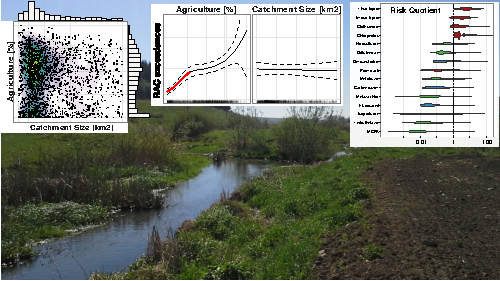
\includegraphics[width=0.7\textwidth]{abstract.pdf}

\end{tocentry}


%%%%%%%%%%%%%%%%%%%%%%%%%%%%%%%%%%%%%%%%%%%%%%%%%%%%%%%%%%%%%%%%%%%%%
\begin{abstract}
% 150-200 words
Small streams are important refugia for biodiversity.
In agricultural areas they may be at high risk from pesticide pollution. 
However, most related studies have been limited to a few streams on the regional level, hampering extrapolation to larger scales. 
We used data from German governmental water quality monitoring to quantify the drivers of pesticide risk and to assess pesticide risk in small streams on a large scale. 
The data set comprised of 1,766,104 measurements related to 24,743 samples in 2,301 sampling sites and of 478 pesticides.  
We investigated the influence of agricultural land use, catchment size, as well as precipitation and seasonal dynamics of pesticide risk using new statistical modeling techniques that explicitly consider the limit of quantification. 
Agricultural land use lead to a 3.4-fold increase in exceedance of risk thresholds once the proportion of agriculture in a catchment exceeded 25 percent. 
Precipitation increased measured pesticide risk by 5\% and was thw highest during summer months.
Risk thresholds were exceeded in 26 percent of small streams, with the highest risk emerging from neonicotinoid insecticides. 
We conclude that pesticides from agricultural land use are a major threat to small streams and their biodiversity, and that governmental pesticide sampling should be adapted to precipitation events. 

% Total words: 197
\end{abstract}

%%%! Check all numbers
%%%! Check all references to supplement


%% -------------------------------------------------------------------------
\section{Introduction}
More than 50\% of the total land area in Germany is used by agriculture \citep{statistisches_bundesamt_bodenflache_2014}.
In the year 2014 more than 45,000 tonnes of 766 authorized pesticides were sold for application on this area \citep{bundesamt_fur_verbraucherschutz_und_lebensmittelsicherheit_absatz_2015}.
The applied pesticides may enter surface waters via spray-drift, edge-off-field run-off or drainage \citep{stehle_probabilistic_2013,schulz_comparison_2001,liess_determination_1999}.
Once entered the surface waters they may have adverse effects on biota and ecosystem functioning \citep{schafer_thresholds_2012}. 
Although it is known that pesticide pollution and its ecological effects increase with the fraction of agricultural land use in the catchment \citep{schulz_field_2004}, the shape of the relationship is unknown and studies on potential thresholds are lacking.

Two recent studies indicate that pesticides might threaten freshwater biodiversity in the European union.
\citet{malaj_organic_2014} analyzed data supplied to the European Union (EU) in the context of the Water Framework Directive (WFD) and showed that almost half of European water bodies are at risk from pesticides.
\citet{stehle_pesticide_2015} compiled 1,566 measured concentrations of 23 insecticides in the EU from scientific publications. 
They found that many of these measurements exceed regulatory acceptable concentrations (RAC).
However, these studies reflect only a small amount of potentially available data (173 sites in predominantly mid-sized and large rivers in \citet{malaj_organic_2014} and 138 measurements in \citet{stehle_pesticide_2015}), and it is unclear how representative they are for Germany. % 173 estimated from digitized figure C.3 in Malaj 2014; Stehle: Table 2.
Much more comprehensive data on thousands of sites are available from national monitoring programs that are setup for the surveillance of water quality,
which is done independently by the federal states in Germany in compliance with the WFD \citep{quevauviller_water_2008} and additional state-specific needs. 
Despite these data providing the opportunity to study pesticide risks and other research questions on a large scale with high spatial density, to date these data have not been compiled and related analyses are lacking. 

Small streams comprise a major fraction of streams \citep{nadeau_hydrological_2007}, accommodate a higher proportion of biodiversity compared to larger freshwater systems \citep{davies_comparison_2008, biggs_report_2014} and play an important role in recolonization of disturbed downstream reaches \citep{liess_analyzing_2005, orlinskiy_forested_2015}.
Nevertheless, a clear definition of SS in terms of catchment or stream size is currently lacking \citep{lorenz_specifics_2016}. 
For example, the WFD defines SS with a catchment size between 10 and 100 km\textsuperscript{2}, without further categorisation of streams \textless 10km\textsuperscript{2} and \citet{lorenz_specifics_2016} defines SS with catchment size \textless 10km\textsuperscript{2}. 

However, small streams might be also at high risk of pesticide contamination from adjacent agricultural areas and lower dilution potential \citep{schulz_field_2004,liess_determination_1999}.
Indeed, meta-analyses using data from studies with a few sites reported higher pesticide pollution in smaller streams compared to bigger streams \citep{stehle_pesticide_2015,schulz_field_2004}.
Despite their ecological relevance and potentially higher pesticide exposure, a recent analysis of pesticide studies showed that a disproportionally small fraction of studies was conducted in small water bodies, and these were largely limited to a few sites \citep{lorenz_specifics_2016}. 
Consequently, knowledge on the pesticide pollution of small streams on larger scales is scant.

In this study we compiled and analyzed large-scale chemical monitoring data from small streams in Germany. 
First, we analysed the shape of the relationship between pesticide risk, agricultural land use and catchment size and examined whether related thresholds for pesticide risks can be derived. 
Second, we investigated the influence of precipitation and seasonal dynamics on pesticide detections, given that precipitation proved an important driver of pesticide exposure in several small-scale studies \citep{wittmer_significance_2010}\citep{schulz_field_2004}, but it is unknown whether a precipitation signal prevails on large scales. 
Finally, we quantified the current risks from pesticides in small streams in Germany.



%% -------------------------------------------------------------------------
\section{Methods}
\subsection{Data compilation}
We requested pesticide monitoring data from sampling sites that can be classified as small streams (catchment sizes $\mathrm{< 100km^2}$ according to the WFD) from all 13 non-city federal states of Germany (see Supplemental Table~S1 for the abbreviations of federal state names). 
The request encompassed only the years 2005 to 2015.
We homogenized and unified all data provided by the federal states into a database and implemented a robust data cleaning workflow (see Supplemental Figure~S1 for details) \citep{poisot_best_2015}.

We identified precipitation at sampling sites by a spatio-temporal intersection of sampling events with gridded daily precipitation data (60$\times$30 arcsec resolution) available from the German Weather service (DWD).
This data spatially interpolates daily precipitation values from local weather stations \citep{rauthe_central_2013}. 
We performed the intersection for the actual sampling date and the day before and extracted precipitation during and up to 48 hours before sampling. 


\subsection{Characterization of catchments}
We compiled a total of 2,369 sampling sites in small streams with pesticide measurements. %see do_overview.R
Alongside, we also requested catchment sizes and percentage agricultural land use within the catchment for the sampling sites from the federal states. %see do_overview.R
Catchment size was available for 59\% of sites from authorities. 
Additionally, we delineated upstream catchments for each of the sampling sites using (i) a digital elevation model (DEM) \citep{eea_digital_2013} and the multiple flow direction algorithm \citep{holmgren_multiple_1994} as implemented in GRASS GIS 7 \citep{neteler_grass_2012} and (ii) from drainage basins provided by the Federal Institute of Hydrology (BfG).
Delineated catchments were visually checked for accuracy by comparison with state stream networks and derived information amalgamated with existing data.
Thus, catchment size information was available for 99\% of all sites (59\% from authorities, 24\% from DEM and 16\% from drainage basins). 

For each derived catchment (either from DEM or drainage basins) we calculated the percentage agricultural land-use within the catchment based on Official Topographical Cartographic Information System (ATKIS) of the land survey authorities \citep{adv_atkis_2016}. 
Thus, agricultural land use information was available for 98\% of all sites (24\% from authorities, 52\% from DEM and 22\% from drainage basins). 
For 97\% of the sites both, the proportion of agricultural land use and catchment size were available. 
68 sites (3\%) lacking these two informations were omitted from the operations outlined below.
%see do_overview.R 



\subsection{Characterization of pesticide pollution}
We characterised pesticide pollution using regulatory acceptable concentrations (RAC) \citep{brock_linking_2010}.
RACs are derived during pesticide authorization as part of the ecological risk assessment.
No unacceptable ecological effect are expected if the environmental concentration remains below this concentration.
\citet{stehle_pesticide_2015} showed that RAC exceedances reflect a decrease in biodiversity and from this perspective are ecologically relevant indicators. 
The German Federal Environmental Agency (UBA) provided RACs for the 105 compounds with highest detection rates (Supplemental Table~S2). 
We expressed RACs as Risk Quotient (RQ):

\begin{equation}
RQ_i = \frac{C_i}{RAC_i}
\end{equation}

where $C_i$ is the concentration of a compound $i$ in a sample.


\subsection{Statistical analyses}
All data-processing and analyses were performed using R \citep{r_core_team_r:_2016}.
To display differences in the spectra of analyzed compounds between federal states we used Multidimensional Scaling (MDS) based on Jaccard dissimilarity in conjunction with complete linkage hierarchical clustering using the vegan package \citep{oksanen_vegan:_2016}.
We determined the optimum number of clusters using the average silhouette width \citep{rousseeuw1987silhouettes}. 

We expected non-linear responses to agriculture and catchment size and therefore, used generalized additive models (GAM) to establish relationships \citep{fewster_analysis_2000}.
We modeled the number of RAC exceedances at a site as:

\begin{align}
\begin{split}
  No(RQ > 1)_i \sim NB(\mu_i, \kappa) \\
  log(\mu_i)= \beta_0 + f_1(agri_i) + f_2(size_i) + log(n_i) \\
\end{split}
\end{align}

where $No(RQ > 1)_i$ is the observed number of RAC exceedances at site $i$. 
We modeled $No(RQ > 1)_i$ as resulting from a negative binomial distribution ($NB$) with mean $\mu_i$ and a quadratic mean-variance-relationship ($Var(No(RQ > 1)_i) = \mu_i + \frac{\mu_i^2}{\kappa}$).
The proportion of agriculture within the catchment ($agri_i$) and the catchment size of the site ($size_i$) were used as predictors of the number of RAC exceedances. 
$f_1$ and $f_2$ are smoothing functions using penalized cubic regression splines \citep{wood_generalized_2006} and $\beta_0$ is the intercept.
The degree of smoothness was estimated using restricted maximum likelihood (REML) during model fitting process \citep{wood_fast_2011}.
The number of measurements per site ($n_i$) was used as an offset to account for differences in sampling efforts (sampling interval and analysed compound spectrum) at a site and is equivalent to modeling the rate of exceedances. 
We used point-wise 95\% Confidence Intervals (CI) of the first derivative of the fitted smooth to check if there are regions of statistically significant changes.
GAMs were fitted using the mgcv package \citep{wood_fast_2011}.

To assess the influence of precipitation and seasonality we modeled the RQ of individual compounds as the response variable.
RQ and concentrations show a skewed distribution with an excess of zeros (no pesticides detected and quantified). 
Therefore, we modeled these as two processes (one generating values below the limit of quantification (LOQ) and one generating values above LOQ) using a Zero-Adjusted Gamma (ZAGA) distribution (Equation~\ref{eqn:eqn3}) \cite{rigby_generalized_2005,stasinopoulos_gamlss.dist:_2016}.
These two processes can be interpreted as changes in the mean value of RQ (change in $\mu$) and changes in the probability of exceeding LOQ and showing any risk (change in $\nu$).

\begin{align}
RQ_i \sim ZAGA(\mu_i, \sigma, \nu_i) = 
  \begin{cases}
    (1 - \nu_i)   & \quad  \text{if } y < LOQ \\
    \nu_i \times f_{Gamma} (\mu_i, \sigma) & \quad \text{if } y \ge LOQ \\
  \end{cases}
  \label{eqn:eqn3}
\end{align}

$\nu_i$ denotes the probability of a measurement i being above LOQ and $f_{Gamma}$ denotes the gamma function and is used for values equal to or greater LOQ, with $\mu$ being the mean and $\sigma$ the standard deviation of RQ.
We used the $log(x+0.05)$ transformed precipitation at sampling date ($log~prec_0$) and the day before ($log~prec_{-1}$), as well as quarters of the year ($Q1-Q4$) as linear predictors for $\mu$ and $\nu$. 
We used appropriate link functions for $\mu$ and $\nu$ and assumed $\sigma$ to be constant. 
Equation~\ref{eqn:eqn4} summarises the deterministic part of the model for a measurement $i$.

\begin{align}
\begin{split}
\log(\mu_{i}) = log~prec_{0 i} + log~prec_{-1 i} + Q1_{i} + Q2_{i}+Q3_{i}+Q4_{i}\\
logit(\nu_{i}) = log~prec_{0 i} + log~prec_{-1 i} + Q1_{i} + Q2_{i}+Q3_{i}+Q4_{i}
\end{split}
\label{eqn:eqn4}
\end{align}

To account for temporal auto-correlation and differences between federal states we used $site$ nested within $state$ as random intercepts.
We implemented this model using the gamlss package \cite{stasinopoulos_generalized_2007}. 

We fitted this model separately to each compound with a RAC, measured in at least 1000 samples and with more than 5\% of values above LOQ (n = 23 compounds, see Supplemental Table~S3 for a list of compounds). 
To summarise the coefficients across the 24 modeled compounds we used a random effect meta-analysis for each model coefficient separately \citep{harrison_getting_2011}, resulting in an averaged effect of the 24 compounds.
The results of individual compounds are provided in the Supplemental Table~S4 and Figure~S7.
The meta-analysis was performed using the metafor package \citep{Viechtbauer_2010}. 



%% -------------------------------------------------------------------------
\section{Results}
\subsection{Overview of the compiled data}

The compiled dataset used in analysis comprised 1,766,104 pesticide measurements of 24,743 samples at 2,301 sampling sites in small streams.  %see do_overview.R for numbers.
These samples were all taken via grab sampling.  
We found large differences in the number of sampling sites between federal states and their spatial distribution (Figure~\ref{fig:fig1} and Supplemental Table~S1). 
The number of small stream sampling sites per state ranged from 1 (Lower Saxonia, NI) to 1139 (North Rhine-Westphalia, NW) and no data from Brandenburg. 

\begin{figure}[ht]
  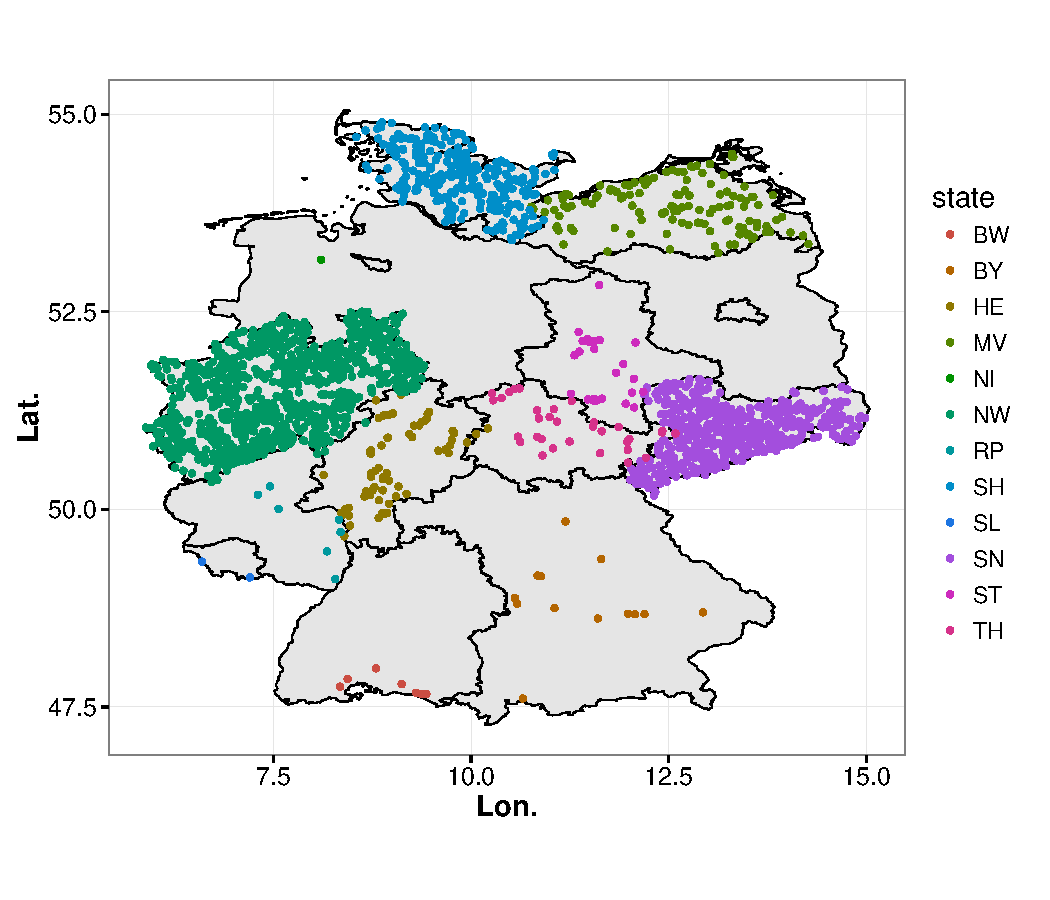
\includegraphics[width=0.6\textwidth]{figure1.pdf}
  \caption{Spatial distribution of the 2,301 small stream sampling sites. Colour codes different federal states, see Supplemental Table~S1 for abbreviations.}
  \label{fig:fig1}
\end{figure}

In total 478 different compounds used as pesticides and their metabolites were measured at least once (Supplemental Table~S2). 
Most of the compounds were herbicides (179), followed by insecticides (117) and fungicides (109). % see overview.R
Most samples were taken in the months April till October, with fewer samples during winter (see Supplemental Figure~S3).
4\% (71,113) of all measurements were detects above LOQ.
We found substantial differences in the spectra of analyzed pesticides between federal states (Figure~\ref{fig:fig2}).
The number of different pesticides per state ranged from 57 (SL) to 236 (RP) (Supplemental Table~S1).
Hierarchical clustering revealed that RP and NI analysed a distinct compound spectra compared to the cluster of other states.
Although there was high variation within the remaining cluster, this could not be further split (Figure~\ref{fig:fig2}, also Supplemental Figures~S4 and S5).

\begin{figure}[ht]
  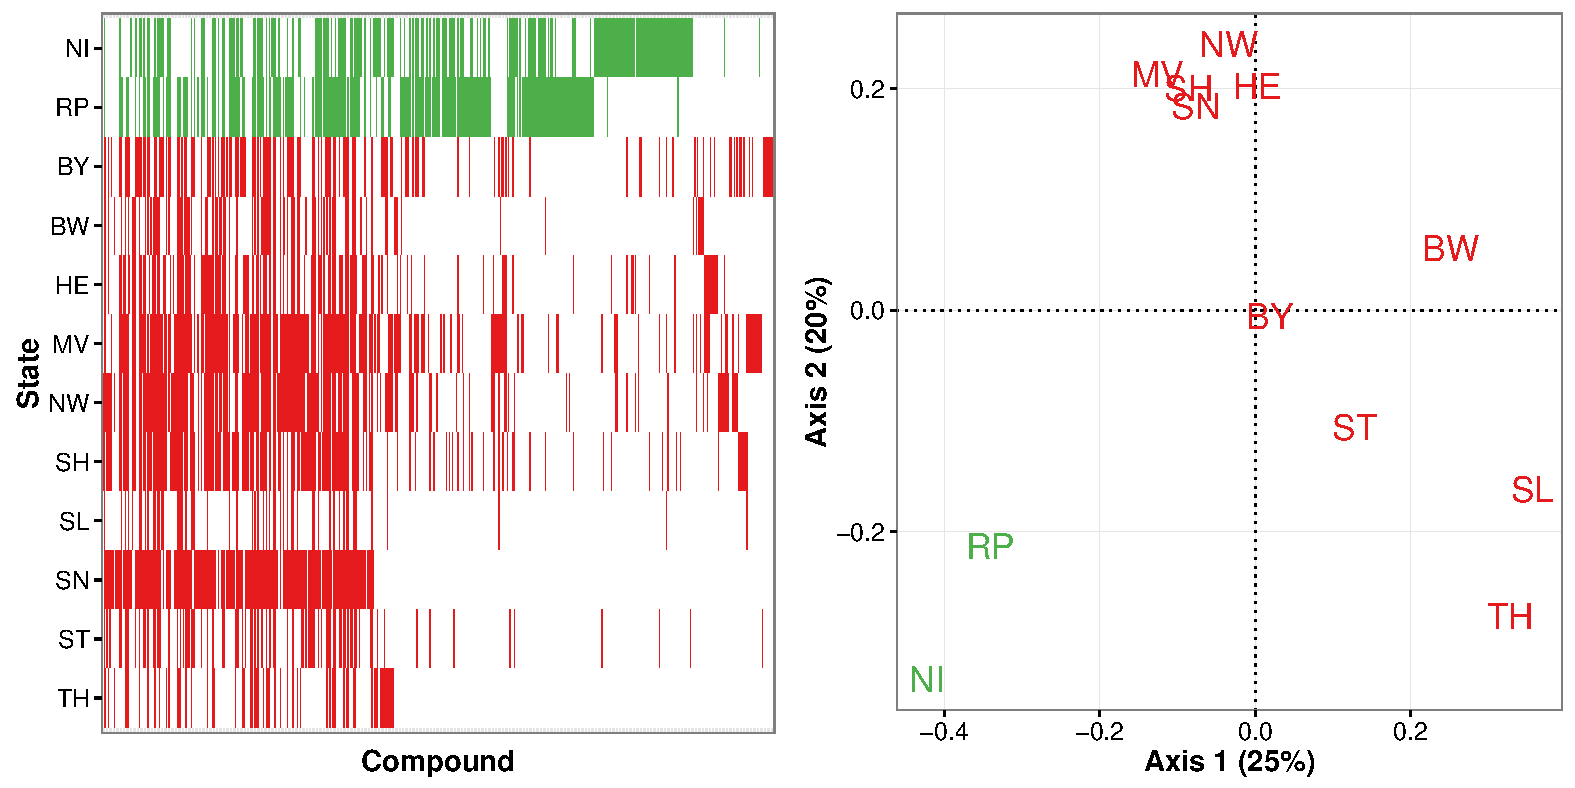
\includegraphics[width=\textwidth]{figure2.pdf}
  \caption{Compound spectra of the different federal states. Left: Barcode plot - each vertical line is an analysed compound. Right: MDS ordination. 
  Colors according to two clusters determined by hierarchical clustering (see Supplemental Figure~S4).}
  \label{fig:fig2}
\end{figure}

The distribution of sampling sites across catchment sizes indicated a disproportionally low number of sites of catchments below $10~km^2$, with
most sampling sites having catchment sizes between 10 and 25 $km^2$ (Figure~\ref{fig:fig3}). 


\begin{figure}[ht]
  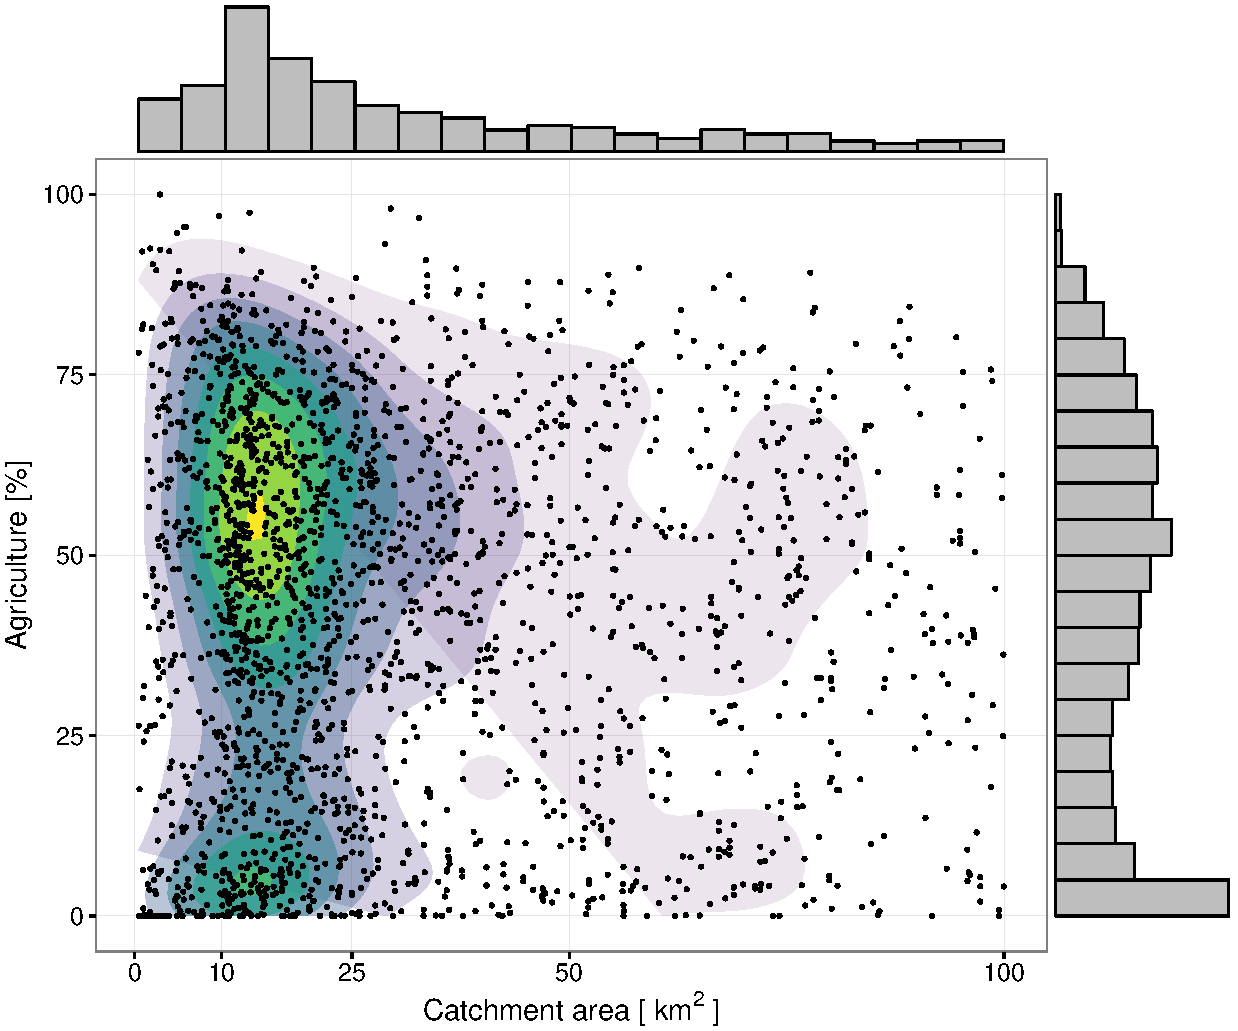
\includegraphics[width=.8\textwidth]{figure3.pdf}
  \caption{Distribution of catchment area and agriculture within the catchment area across the sampling sites.
  Colour codes the 2-dimensional density of points.}
  \label{fig:fig3}
\end{figure}


\subsection{Influence of agricultural land use and catchment size}
The number of RAC exceedances increased strongly and statistically significant up to 25\% agriculture within the catchment.
The mean number of RAC exceedances per site increased strongly and statistically significant from 0.13 (no agriculture) to 0.44 (25\% agriculture within the catchment). 
Above this threshold the exceedances leveled.
Above 75\% agriculture within the catchment the number of exceedances further increased, but the increase was not statistically significant (Figure~\ref{fig:fig4}, left). 
Catchment size had no statistically significant effect on the number of RAC exceedances (Figure~\ref{fig:fig4}, right).
We also could not detect a statistically significant interaction between catchment size and agriculture. 

\begin{figure}[ht]
  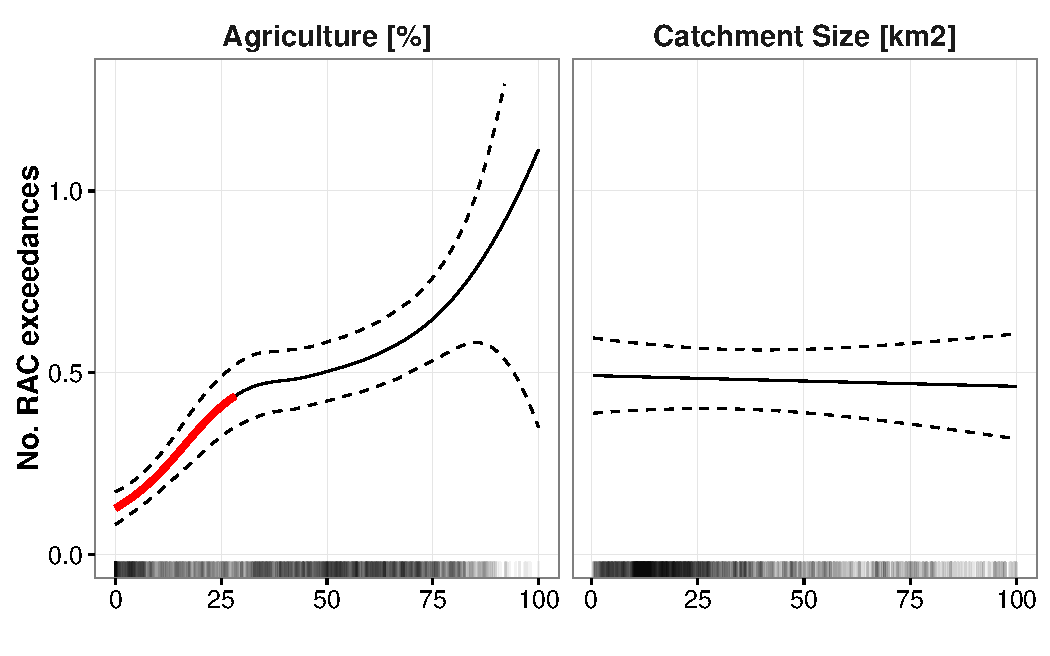
\includegraphics[width=0.95\textwidth]{figure4.pdf}
  \caption{Effect of percent agriculture within the catchment (left) and catchment size (right) on the number of RAC exceedances. Red line marks statistically significant changes. Dashed lines denote 95\% point-wise Confidence Intervals.
  }
  \label{fig:fig4}
\end{figure}


\subsection{Effect of precipitation on pesticide risk}
The spatio-temporal intersection revealed that most samples were taken during periods of low precipitation.
For example, only 5\% of the samples were taken at or after days with rainfall events greater than 10mm / day (Supplemental Figure~S6). 

$prec_{0}$ and $prec_{-1}$ increased the probability of exceeding LOQ and the mean value of RQ.
An increase of precipitation in $Q2$ before sampling ($prec_{-1}$) from 1mm to 10mm precipitation lead to a 5\% higher mean RQ and the probability to exceed LOQ increases from 4\% to 6\% on average (Figure~\ref{fig:fig5}, top). % do_precip.R
Effects on individual compounds are provided in the Supplemental Table~S4.
Precipitation before sampling ($prec_{-1}$) had a stronger effect than precipitation during sampling ($prec_{0}$). 
This difference was less pronounced for the mean value of RQ (Figure~\ref{fig:fig5}, top). 

The first quarter showed the lowest RQ and probability of exceeding LOQ.
Both increased during summer months and decreased towards the end of the year.
There was a probability of 4\% to exceed LOQ in $Q1$ and 10\% in $Q2$.
The differences were less pronounced for the mean value of RQ and with less precision (Figure~\ref{fig:fig5}, bottom). 
Individual compounds showed different temporal patterns (see Supplemental Table~S4).


\begin{figure}[ht]
  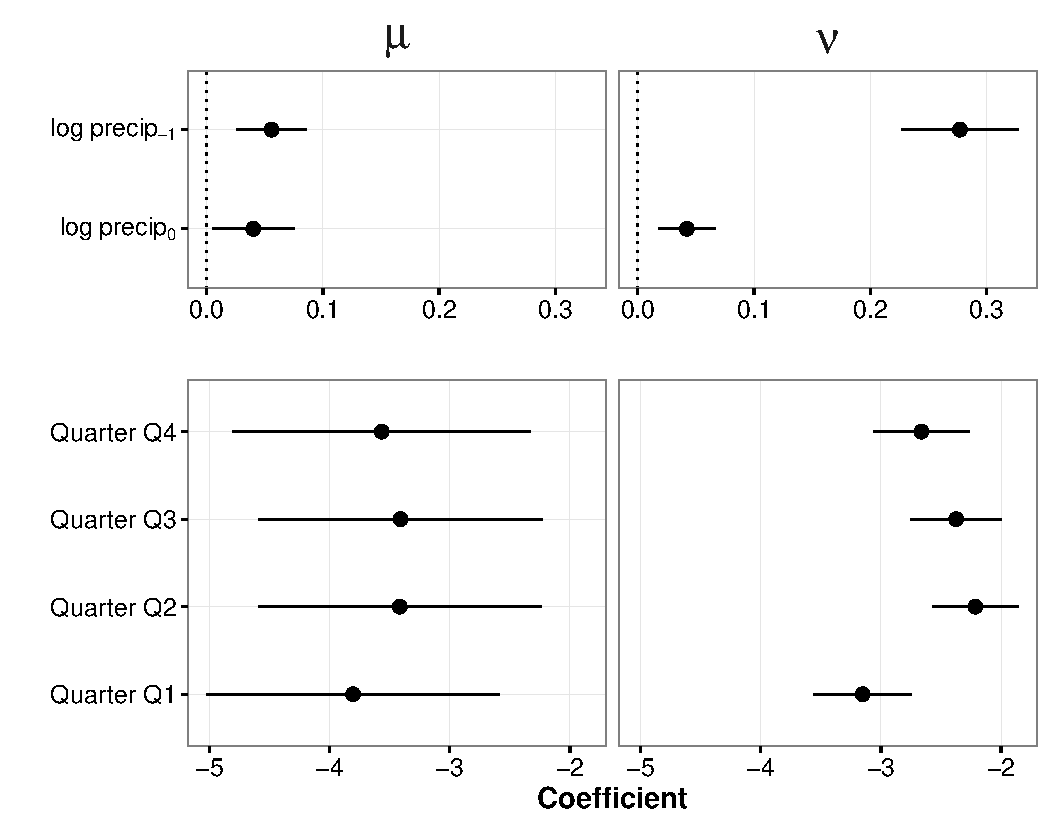
\includegraphics[width=0.8\textwidth]{figure5.pdf}
  \caption{Summarised coefficients (and their 95\% CI) for precipitation (top row) and quarter (bottom row) from a meta-anaylsis of the 24 modeled compounds. Left column: coefficients for mean RQ ($\mu$), right column: coefficients for probabilty to exceeed LOQ ($\nu$). 
  Coefficients are shown on the link scale (see Eq.~\ref{eqn:eqn4}).
  Single compound coefficients are provided in the Supplemental Table~S4 and Figure~S7).
  }
  \label{fig:fig5}
\end{figure}



\subsection{Pesticide risk in small streams}
We found RQ > 1 in 26\% of sampling sites and RQ > 0.1 in 54\% of sites. 
In 23\% of sites chemicals with RAC were never detected (see also Supplemental Figure~S8).
Neonicotinoid insecticides and Chlorpyrifos showed the highest RQ (Figure~\ref{fig:fig6}). %do_pollution.R
For Thiacloprid and Chlorpyrifos the RAC was less than LOQ, therefore, all detections have an RQ~\textgreater~1. 
The herbicides Nicosulfuron and Diflufenican, as well as the fungicide Dimoxystrobin also showed high exceedances of RQ (26.7, 14.1 and 21.1 \% of measurements~\textgreater~LOQ).
RAC exceedances were found in 15\% of samples with detects (and 7.7\% of all samples with RAC).

The highest RQ were observed for Chlorpyrifos (max(RQ) = 244), Clothianidin (max(RQ) = 157), Dimoxystrobin(max(RQ) = 117) and Isoproturon (max(RQ) = 80). 
Where analysed, metabolites exhibited the highest detection rates (for example, Metazachlor sulfonic acid was detected in 84\% of all samples were it was analysed (n = 3038, see also Supplemental Figure~S9).
Glyphosate was the compound with the highest detection rates (41\%, n = 3557 samples), followed by Boscalid (23\%, n = 9886) and Isoproturon (22\%, n = 19112). 
However, only the latter showed RQ exceedances (Figure~\ref{fig:fig6}).
In 45.9\% of samples more than one compound was quantified, with a maximum of 54 different compounds in one sample (Supplemental Figure~S8). 

\begin{figure}[ht]
  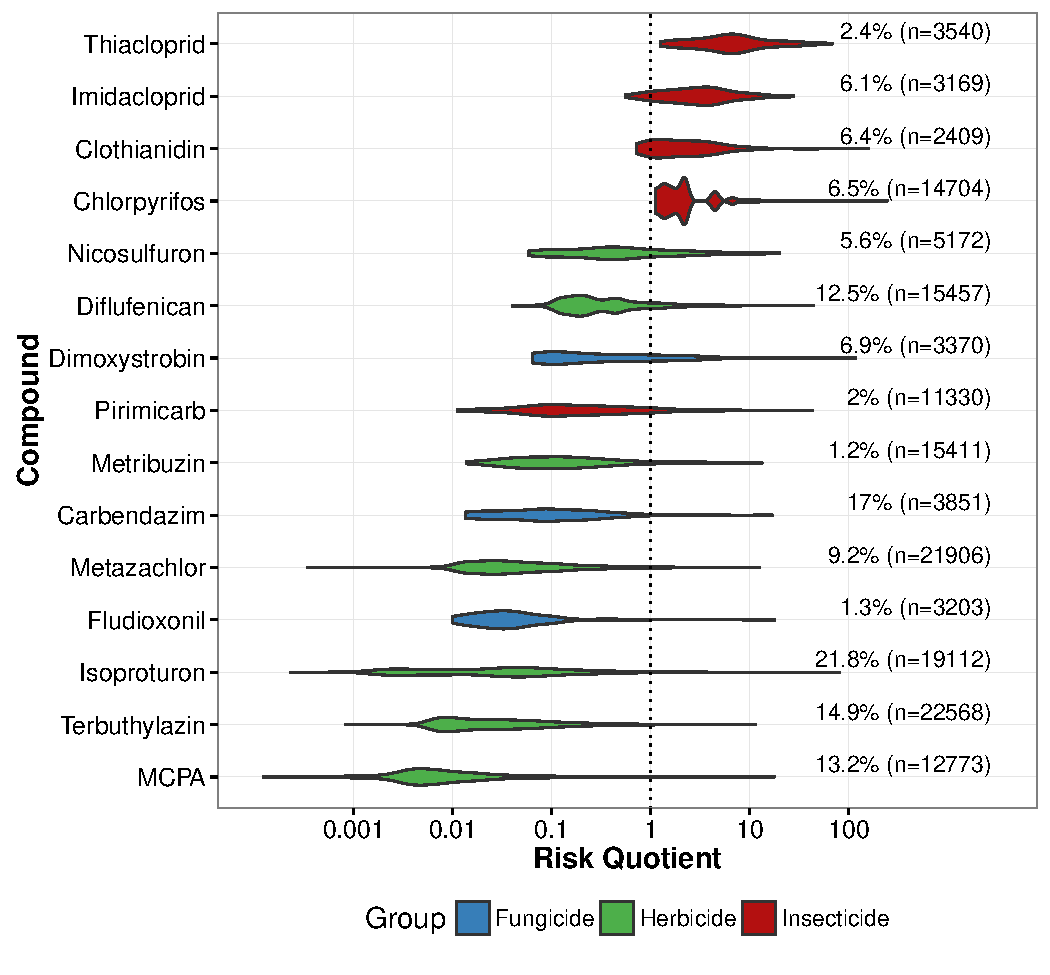
\includegraphics[width=0.6\textwidth]{figure6.pdf}
  \caption{15 compounds with the highest risk quotients in small streams. Non-detects are not shown due to the logarithmic axis. Numbers on the right give the percentage of values \textgreater LOQ and the total number of samples were the compound was analysed.
  }
  \label{fig:fig6}
\end{figure}




%% -------------------------------------------------------------------------
\section{Discussion}
\subsection{Overview on the compiled dataset}
The compiled dataset of governmental monitoring data, with a particular focus on small streams, represents currently the most comprehensive one available for Germany.
Similar nationwide datasets have been compiled for the Netherlands \citep{vijver_spatial_2008}, Switzerland \citep{munz_pestizidmessungen_2011} and the United States \citep{stone2014pesticides}.
While the compilations from Europe are of similar quantity and quality to the  data compiled and analysed here for Germany, the compilation used in \citet{stone2014pesticides} is much smaller.
Nevertheless, there might more data for the United States available (e.g. from Water Quality Portal (WQP), \url{www.waterqualitydata.us}). 

% current problems in monitoring and possible solutions
A nation-wide assessment of pesticide pollution is hampered by the inhomogeneity of monitoring data between federal states:
Beside large differences in the spatial distribution and quantity of sampling sites (Figure~\ref{fig:fig1}), the spectrum of analyzed compounds (Figure~\ref{fig:fig2}) and the quality of chemical analyses differed between states. 
Although, the outlined differences between states, all ecoregions occurring Germany \citep{illies1978limnofauna,abell2008freshwater} are covered by the presented dataset and therefore, may represent a sample of all small streams in Central Europe. 
For Thiacloprid and Chlorpyrifos the LOQs were above the RAC, which means that some exceedances were likely not detected.
For these compounds a lowering of LOQ is essential for reliable assessment.
Moreover, a nation-wide assessment would benefit from a harmonized spectrum of analysed compounds between federal states. 

Given their high abundance in the landscape \citep{nadeau_hydrological_2007} small streams are underrepresented in the current monitoring (Figure~\ref{fig:fig3}). 
Especially, sampling sites in streams below 10~km\textsuperscript{2} are disproportionally low, which may be attributed to the missing categorisation in the WFD. 
Clearly, there is currently a lack of knowledge for these small streams.
We analysed only data from small streams, however, for lentic small water bodies this lack might be even greater \citep{lorenz_specifics_2016}. 



\subsection{Influence of agricultural land use and catchment size}
% agriculture
We found a strong influence of agriculture on the pollution of streams.
If there is more the 25\% agriculture within a catchment pesticides, it is likely that a RAC will be exceeded, with a further increase in fully agricultural catchments (above 75 \% agriculture).
To our knowledge, this is the first study investigating such thresholds of pesticide risk.
Previous studies examined thresholds for percent agricultural land use with respect to the response of biological communities, integrating different agricultural stressors.
\citet{feld_response_2013} found change points of biological community metrics at 40\% agricultural land use in lowland streams in Europe.
Similarly, \citet{waite_agricultural_2014} found a threshold for aquatic diatoms at 40\% agricultural land use in wadeable streams in the United States.
Our results coincide with these thresholds and suggest that pesticides might contribute to the observed biological changes. 

% size
We did not find a relationship between pesticide pollution and catchment size.
However, previous studies showed that small streams are more polluted that bigger streams \citep{schulz_field_2004,stehle_pesticide_2015,knauer_pesticides_2016}.
This can be explained by the relatively short gradient of catchment sizes in our dataset, with most of the streams with catchments above $10~km^2$ and below $100~km^2$ (Figure~\ref{fig:fig3}, top).
For example, the gradient of \citet{schulz_field_2004} covered 6 orders of magnitude.


\subsection{Effect of precipitation on pesticide risk}
Our results revealed that pesticide sampling for chemical monitoring in Germany is mainly performed when no precipitation occurs. 
Nevertheless, we found a 5\% higher RQ if samples were taken after rainfall events. 
Samples taken at the day of a rainfall event showed less risk than samples taken one day after a rainfall event.
This could be explained by a sampling just before the actual rainfall event.
Pesticide concentrations in agricultural small streams generally show short-term peak concentrations \citep{wittmer_significance_2010}, therefore, a sampling at the day after a rainfall-event might miss peak concentrations.
The effects of precipitation were more pronounced for the probability to exceed LOQ, with smaller effect sizes for RQ.
This could be attributed to a higher variability of absolute concentrations.
Overall, our results indicate that current pesticide monitoring relying on grab sampling, largely disconnected from precipitation events, considerably underestimates pesticide risks.
Automatic event-drive samplers \citep{stehle_probabilistic_2013} and passive samplers \citep{fernandez_calibration_2014,moschet_evaluation_2015} may help overcome these shortcomings and provide a better representation, especially for small water bodies \citep{lorenz_specifics_2016}. 

We found highest the probability of exceeding LOQ during summer (10\% for Q2) and lowest in the first quarter (4\%, Figure~\ref{fig:fig5}, bottom right).
This yearly pattern coincides with their main application season for pesticides in Central Europe.
Nevertheless, there are compound specific differences in the yearly pattern, which explains the wide CI for the absolute RQ (Figure~\ref{fig:fig5}, bottom left).
For example, the herbicide Diflufenican showed highest RQ and probability of exceeding LOQ during the winter quarters Q1 and Q4 (Supplemental Table~S4), which coincides with the application period it is registered for in Germany \citep{bvl_online_2016}.
Our study suggests that pesticide risks display compound specific spatio-temporal dynamics.
Currently, little is known about these and further research on those might provide useful information for future ecological risk assessment. 
For example, the sensitivity of organisms is often life stage dependent \citep{hutchinson1998analysis} and knowledge on temporal dynamics could inform on concurrent exposure to multiple pesticides, as well as assist to parameterise toxicokinetic and toxicodynamic models \citep{ashauer2016modelling}. 


\subsection{Pesticides in small streams}
Our results suggest that small streams are frequently exposed to ecologically relevant pesticide concentrations.
In one quarter of small streams RACs were exceeded at least once.
\citet{stehle_pesticide_2015} found the highest percentage of RAC exceedances for organophosphate insecticides. 
By contrast, we found that that neonicotinoid insecticides have highest exceedances of RACs, followed by the organophosphate chlorpyrifos. 
This difference can be attributed to the low sample size for neonicotinoid insecticides in their study (n = 33) compared to the dataset presented here (for example 3,540 samples of Thiacloprid, Figure~\ref{fig:fig6}). 
Overall, our results suggest that neonicotinoids may currently pose a high risk to freshwater ecosystems. 
Our results add further evidence to the growing literature on risks arising from neonicotinoids for aquatic \citep{morrissey2015neonicotinoid} and terrestrial ecosystems \citep{pisa2015effects}.

Compared to \citet{stehle_pesticide_2015} we found lower rates RAC exceedances (15\% (n = 12,615) vs 44\% (n = 1,566) of samples with measurements above LOQ). 
This may be attributed to two differences: i) Different objectives of governmental monitoring and scientific studies. Scientific studies may be slightly biased towards streams with high pollution to detect effects, whereas monitoring aims mainly at spatially representative surveillance of water quality, also during periods of lower pesticide usage and at natural sites. ii) Different sampling strategies. The dataset compiled here comprised only samples from grab sampling, which may considerably underestimate pesticide exposure \citep{stehle_probabilistic_2013}. 

By contrast, \citet{knauer_pesticides_2016} found exceedances from monitoring data mainly for herbicides and fungicides and only one insecticide Chlorpyrifos.
However, RAC exceedances were generally lower and less abundant compared to our results from Germany. 
This might reflect differences in pesticide use between countries and ecoregions. 
From the definition of RAC it follows that if the concentration of a compound exceeds its RAC ecological effects are expected.
Indeed, \citet{stehle_agricultural_2015} found that biological diversity of stream invertebrates was significantly reduced by 30\% at RQ = 1.12 and by 10\% at 1/10 of RAC.
We found RQ values greater than 1.12 in one quarter of small streams and RQ at 1/10 of RAC in more the half of streams. 
Consequently, we conclude that on a large-scale agricultural pesticides are a major threat to small streams, the biodiversity they host and the services they provide. 
This threat may exacerbate because pesticides often occur in mixtures \cite{schreiner_pesticide_2016} and may co-occur with other stressors \citep{schafer_contribution_2016}.

% Approval / Risk Assessment
Monitoring data, despite the outlined limitations, provides an opportunity to study large-scale environmental occurrence patterns of pesticides.
Nevertheless, such nationwide compilations, may not only be used for governmental surveillance, but also to answer other questions, like validation of exposure modeling \cite{knabel_fungicide_2014}, retrospective evaluation of regulatory risk assessment \citep{knauer_pesticides_2016,stehle_pesticide_2015}or occurrences of pesticide mixtures \cite{schreiner_pesticide_2016}, though the sampling design need to account for precipitation events to provide robust data. 
Our results suggest that exceedances of RACs are landscape dependent % = Zusammenhang RAC<->Agriculture
and therefore, landscape features should be taken into account in the registration process of pesticides.
Moreover, the high exceedances of RAC indicate that the authorisation process for pesticides may require further development. 





%%%%%%%%%%%%%%%%%%%%%%%%%%%%%%%%%%%%%%%%%%%%%%%%%%%%%%%%%%%%%%%%%%%%%
\begin{acknowledgement}
The authors thank the federal state authorities for providing chemical monitoring data and the German Federal Environmental Protection Agency (UBA) for funding a related project (FKZ 3714 67 4040 / 1). 
\end{acknowledgement}


%%% Word count
% abstract    :  200
% 4 big(600)  : 2400
% 2 small(300):  600
% acknowledg  :   30
%              =====
% subtotal      3227
% text body   : 3700
% ======================================
% total       : 6930

%%%%%%%%%%%%%%%%%%%%%%%%%%%%%%%%%%%%%%%%%%%%%%%%%%%%%%%%%%%%%%%%%%%%%
\begin{suppinfo}
The following files are available free of charge.
\begin{itemize}
  \item Supplemental\_Materials.pdf : Supplemental Materials (Figures, Tables, Models).
\end{itemize}
\end{suppinfo}


%%%%%%%%%%%%%%%%%%%%%%%%%%%%%%%%%%%%%%%%%%%%%%%%%%%%%%%%%%%%%%%%%%%%%
\bibliography{references}

\end{document}
